\documentclass[11pt,a4paper]{article}
\usepackage[margin=1.25cm, top=1.1cm, bottom=1.2cm]{geometry}
\usepackage[scaled]{helvet}\renewcommand\familydefault{\sfdefault}
\usepackage[T1]{fontenc}
\usepackage{tikz,xcolor,array,tabularx,booktabs,enumitem,multicol}
\usetikzlibrary{arrows.meta,shapes.misc,calc}
\pagestyle{empty}\setlength{\parindent}{0pt}
\definecolor{ttdark}{HTML}{2B2D5C}
\definecolor{ttaccent}{HTML}{D9480F}
\definecolor{ttglow}{HTML}{25B5A4}
\definecolor{ttpale}{HTML}{EEF1FA}
\tikzset{flag/.style={draw=ttaccent, fill=white, text=ttaccent, line width=0.8pt, font=\tiny\bfseries, rounded corners=2pt, inner sep=2pt, align=center}}
\newcommand{\banner}[1]{{\color{ttdark}\large\bfseries #1}\par\vspace{-7pt}{\color{ttdark}\rule{\linewidth}{1.2pt}}\par\vspace{-2pt}}
% time machine dial: \dial{BACK|FORWARD}{amount}{unit}
\newcommand{\dial}[3]{\tikz[baseline=-3.5pt]{\node[draw=ttdark, line width=1pt, rounded corners=3pt, inner sep=1.5pt] {%
  \tikz[baseline]{\node[draw=black!45, text=ttdark, font=\scriptsize\bfseries, inner sep=2.5pt, minimum width=1.5cm]{#1};}\,%
  \tikz[baseline]{\node[draw=black!45, text=black, font=\scriptsize\bfseries, inner sep=2.5pt, minimum width=1.3cm]{#2};}\,%
  \tikz[baseline]{\node[draw=black!45, text=ttdark, font=\scriptsize\bfseries, inner sep=2.5pt, minimum width=1.6cm]{#3};}};}}
\newcommand{\aline}{\rule{2.6cm}{0.4pt}}
\newcommand{\lline}{\rule{4.6cm}{0.4pt}}
\newcommand{\ans}[1]{\textcolor{red!75!black}{\bfseries #1}}
\newcommand{\factbox}[2]{\begin{tikzpicture}\node[draw=ttdark, rounded corners=4pt, line width=1pt, inner sep=7pt, text width=#1, align=left, font=\small]{#2};\end{tikzpicture}}
\begin{document}


\begin{tikzpicture}
\node[draw=ttdark, line width=1.5pt, rounded corners=6pt, minimum width=\linewidth, minimum height=1.9cm] (h) {};
\node[text=ttdark, font=\fontsize{30}{32}\selectfont\bfseries, anchor=west] at ($(h.west)+(0.5,0.18)$) {Time Travellers!};
\node[text=ttaccent, font=\small\bfseries, anchor=west] at ($(h.west)+(0.55,-0.6)$) {Calendars, conversions and timelines};
\begin{scope}[shift={($(h.east)+(-1.4,0)$)}]
\draw[ttdark, line width=1.5pt] (0,0) circle (0.72); \foreach \a in {0,30,...,330} \draw[ttdark] (\a:0.58) -- (\a:0.72);
\draw[ttdark, line width=2pt, -{Stealth[length=4pt]}] (0,0) -- (115:0.42); \draw[ttdark, line width=1.2pt, -{Stealth[length=4pt]}] (0,0) -- (-160:0.6);
\draw[ttaccent, line width=1.8pt, -{Stealth[length=6pt]}] (40:0.95) arc (40:-200:0.95);
\end{scope}
\end{tikzpicture}\par\medskip
\banner{Part A \quad Calendar hops --- small jumps}\par\smallskip
{\small Dr Chrono's time machine is parked in the school car park. \textbf{It is Saturday 31 October 2026, 10:00} (circled). For each dial setting, use the calendars to find where the machine lands if Dr Chrono travels from Saturday 31 October 2026, 10:00.}\par\medskip
\begin{center}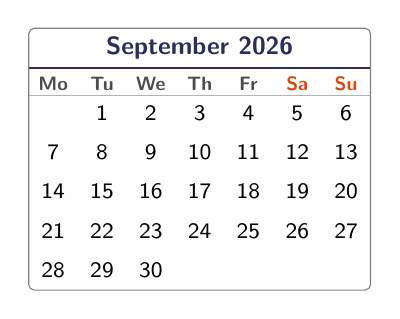
\begin{tikzpicture}[x=0.62cm,y=0.50cm,baseline=(current bounding box.north)]
\node[text=ttdark, font=\bfseries\small] at (3.5,0.65) {September 2026}; \draw[ttdark, thick] (0,0.15) -- (7,0.15);
\node[font=\scriptsize\bfseries, text=black!70] at (0.5,-0.25) {Mo};
\node[font=\scriptsize\bfseries, text=black!70] at (1.5,-0.25) {Tu};
\node[font=\scriptsize\bfseries, text=black!70] at (2.5,-0.25) {We};
\node[font=\scriptsize\bfseries, text=black!70] at (3.5,-0.25) {Th};
\node[font=\scriptsize\bfseries, text=black!70] at (4.5,-0.25) {Fr};
\node[font=\scriptsize\bfseries, text=ttaccent] at (5.5,-0.25) {Sa};
\node[font=\scriptsize\bfseries, text=ttaccent] at (6.5,-0.25) {Su};
\node[font=\footnotesize] at (1.5,-1.0) {1};
\node[font=\footnotesize] at (2.5,-1.0) {2};
\node[font=\footnotesize] at (3.5,-1.0) {3};
\node[font=\footnotesize] at (4.5,-1.0) {4};
\node[font=\footnotesize] at (5.5,-1.0) {5};
\node[font=\footnotesize] at (6.5,-1.0) {6};
\node[font=\footnotesize] at (0.5,-2.0) {7};
\node[font=\footnotesize] at (1.5,-2.0) {8};
\node[font=\footnotesize] at (2.5,-2.0) {9};
\node[font=\footnotesize] at (3.5,-2.0) {10};
\node[font=\footnotesize] at (4.5,-2.0) {11};
\node[font=\footnotesize] at (5.5,-2.0) {12};
\node[font=\footnotesize] at (6.5,-2.0) {13};
\node[font=\footnotesize] at (0.5,-3.0) {14};
\node[font=\footnotesize] at (1.5,-3.0) {15};
\node[font=\footnotesize] at (2.5,-3.0) {16};
\node[font=\footnotesize] at (3.5,-3.0) {17};
\node[font=\footnotesize] at (4.5,-3.0) {18};
\node[font=\footnotesize] at (5.5,-3.0) {19};
\node[font=\footnotesize] at (6.5,-3.0) {20};
\node[font=\footnotesize] at (0.5,-4.0) {21};
\node[font=\footnotesize] at (1.5,-4.0) {22};
\node[font=\footnotesize] at (2.5,-4.0) {23};
\node[font=\footnotesize] at (3.5,-4.0) {24};
\node[font=\footnotesize] at (4.5,-4.0) {25};
\node[font=\footnotesize] at (5.5,-4.0) {26};
\node[font=\footnotesize] at (6.5,-4.0) {27};
\node[font=\footnotesize] at (0.5,-5.0) {28};
\node[font=\footnotesize] at (1.5,-5.0) {29};
\node[font=\footnotesize] at (2.5,-5.0) {30};
\draw[black!30] (0,-0.55) -- (7,-0.55);
\draw[black!50, rounded corners=2pt] (0,-5.5) rectangle (7,1.15);
\end{tikzpicture}\hfill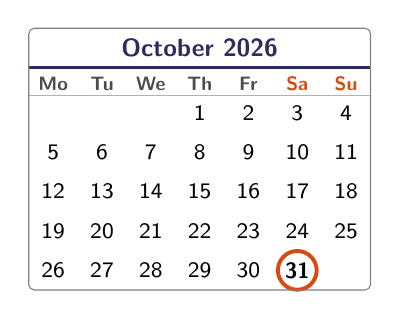
\begin{tikzpicture}[x=0.62cm,y=0.50cm,baseline=(current bounding box.north)]
\node[text=ttdark, font=\bfseries\small] at (3.5,0.65) {October 2026}; \draw[ttdark, thick] (0,0.15) -- (7,0.15);
\node[font=\scriptsize\bfseries, text=black!70] at (0.5,-0.25) {Mo};
\node[font=\scriptsize\bfseries, text=black!70] at (1.5,-0.25) {Tu};
\node[font=\scriptsize\bfseries, text=black!70] at (2.5,-0.25) {We};
\node[font=\scriptsize\bfseries, text=black!70] at (3.5,-0.25) {Th};
\node[font=\scriptsize\bfseries, text=black!70] at (4.5,-0.25) {Fr};
\node[font=\scriptsize\bfseries, text=ttaccent] at (5.5,-0.25) {Sa};
\node[font=\scriptsize\bfseries, text=ttaccent] at (6.5,-0.25) {Su};
\node[font=\footnotesize] at (3.5,-1.0) {1};
\node[font=\footnotesize] at (4.5,-1.0) {2};
\node[font=\footnotesize] at (5.5,-1.0) {3};
\node[font=\footnotesize] at (6.5,-1.0) {4};
\node[font=\footnotesize] at (0.5,-2.0) {5};
\node[font=\footnotesize] at (1.5,-2.0) {6};
\node[font=\footnotesize] at (2.5,-2.0) {7};
\node[font=\footnotesize] at (3.5,-2.0) {8};
\node[font=\footnotesize] at (4.5,-2.0) {9};
\node[font=\footnotesize] at (5.5,-2.0) {10};
\node[font=\footnotesize] at (6.5,-2.0) {11};
\node[font=\footnotesize] at (0.5,-3.0) {12};
\node[font=\footnotesize] at (1.5,-3.0) {13};
\node[font=\footnotesize] at (2.5,-3.0) {14};
\node[font=\footnotesize] at (3.5,-3.0) {15};
\node[font=\footnotesize] at (4.5,-3.0) {16};
\node[font=\footnotesize] at (5.5,-3.0) {17};
\node[font=\footnotesize] at (6.5,-3.0) {18};
\node[font=\footnotesize] at (0.5,-4.0) {19};
\node[font=\footnotesize] at (1.5,-4.0) {20};
\node[font=\footnotesize] at (2.5,-4.0) {21};
\node[font=\footnotesize] at (3.5,-4.0) {22};
\node[font=\footnotesize] at (4.5,-4.0) {23};
\node[font=\footnotesize] at (5.5,-4.0) {24};
\node[font=\footnotesize] at (6.5,-4.0) {25};
\node[font=\footnotesize] at (0.5,-5.0) {26};
\node[font=\footnotesize] at (1.5,-5.0) {27};
\node[font=\footnotesize] at (2.5,-5.0) {28};
\node[font=\footnotesize] at (3.5,-5.0) {29};
\node[font=\footnotesize] at (4.5,-5.0) {30};
\node[circle, draw=ttaccent, line width=1.4pt, inner sep=0pt, minimum size=14pt] at (5.5,-5.0) {};
\node[font=\footnotesize\bfseries, text=black] at (5.5,-5.0) {31};
\draw[black!30] (0,-0.55) -- (7,-0.55);
\draw[black!50, rounded corners=2pt] (0,-5.5) rectangle (7,1.15);
\end{tikzpicture}\hfill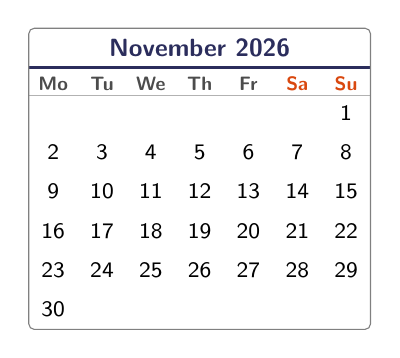
\begin{tikzpicture}[x=0.62cm,y=0.50cm,baseline=(current bounding box.north)]
\node[text=ttdark, font=\bfseries\small] at (3.5,0.65) {November 2026}; \draw[ttdark, thick] (0,0.15) -- (7,0.15);
\node[font=\scriptsize\bfseries, text=black!70] at (0.5,-0.25) {Mo};
\node[font=\scriptsize\bfseries, text=black!70] at (1.5,-0.25) {Tu};
\node[font=\scriptsize\bfseries, text=black!70] at (2.5,-0.25) {We};
\node[font=\scriptsize\bfseries, text=black!70] at (3.5,-0.25) {Th};
\node[font=\scriptsize\bfseries, text=black!70] at (4.5,-0.25) {Fr};
\node[font=\scriptsize\bfseries, text=ttaccent] at (5.5,-0.25) {Sa};
\node[font=\scriptsize\bfseries, text=ttaccent] at (6.5,-0.25) {Su};
\node[font=\footnotesize] at (6.5,-1.0) {1};
\node[font=\footnotesize] at (0.5,-2.0) {2};
\node[font=\footnotesize] at (1.5,-2.0) {3};
\node[font=\footnotesize] at (2.5,-2.0) {4};
\node[font=\footnotesize] at (3.5,-2.0) {5};
\node[font=\footnotesize] at (4.5,-2.0) {6};
\node[font=\footnotesize] at (5.5,-2.0) {7};
\node[font=\footnotesize] at (6.5,-2.0) {8};
\node[font=\footnotesize] at (0.5,-3.0) {9};
\node[font=\footnotesize] at (1.5,-3.0) {10};
\node[font=\footnotesize] at (2.5,-3.0) {11};
\node[font=\footnotesize] at (3.5,-3.0) {12};
\node[font=\footnotesize] at (4.5,-3.0) {13};
\node[font=\footnotesize] at (5.5,-3.0) {14};
\node[font=\footnotesize] at (6.5,-3.0) {15};
\node[font=\footnotesize] at (0.5,-4.0) {16};
\node[font=\footnotesize] at (1.5,-4.0) {17};
\node[font=\footnotesize] at (2.5,-4.0) {18};
\node[font=\footnotesize] at (3.5,-4.0) {19};
\node[font=\footnotesize] at (4.5,-4.0) {20};
\node[font=\footnotesize] at (5.5,-4.0) {21};
\node[font=\footnotesize] at (6.5,-4.0) {22};
\node[font=\footnotesize] at (0.5,-5.0) {23};
\node[font=\footnotesize] at (1.5,-5.0) {24};
\node[font=\footnotesize] at (2.5,-5.0) {25};
\node[font=\footnotesize] at (3.5,-5.0) {26};
\node[font=\footnotesize] at (4.5,-5.0) {27};
\node[font=\footnotesize] at (5.5,-5.0) {28};
\node[font=\footnotesize] at (6.5,-5.0) {29};
\node[font=\footnotesize] at (0.5,-6.0) {30};
\draw[black!30] (0,-0.55) -- (7,-0.55);
\draw[black!50, rounded corners=2pt] (0,-6.5) rectangle (7,1.15);
\end{tikzpicture}\hfill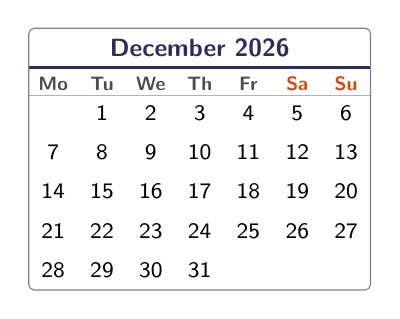
\begin{tikzpicture}[x=0.62cm,y=0.50cm,baseline=(current bounding box.north)]
\node[text=ttdark, font=\bfseries\small] at (3.5,0.65) {December 2026}; \draw[ttdark, thick] (0,0.15) -- (7,0.15);
\node[font=\scriptsize\bfseries, text=black!70] at (0.5,-0.25) {Mo};
\node[font=\scriptsize\bfseries, text=black!70] at (1.5,-0.25) {Tu};
\node[font=\scriptsize\bfseries, text=black!70] at (2.5,-0.25) {We};
\node[font=\scriptsize\bfseries, text=black!70] at (3.5,-0.25) {Th};
\node[font=\scriptsize\bfseries, text=black!70] at (4.5,-0.25) {Fr};
\node[font=\scriptsize\bfseries, text=ttaccent] at (5.5,-0.25) {Sa};
\node[font=\scriptsize\bfseries, text=ttaccent] at (6.5,-0.25) {Su};
\node[font=\footnotesize] at (1.5,-1.0) {1};
\node[font=\footnotesize] at (2.5,-1.0) {2};
\node[font=\footnotesize] at (3.5,-1.0) {3};
\node[font=\footnotesize] at (4.5,-1.0) {4};
\node[font=\footnotesize] at (5.5,-1.0) {5};
\node[font=\footnotesize] at (6.5,-1.0) {6};
\node[font=\footnotesize] at (0.5,-2.0) {7};
\node[font=\footnotesize] at (1.5,-2.0) {8};
\node[font=\footnotesize] at (2.5,-2.0) {9};
\node[font=\footnotesize] at (3.5,-2.0) {10};
\node[font=\footnotesize] at (4.5,-2.0) {11};
\node[font=\footnotesize] at (5.5,-2.0) {12};
\node[font=\footnotesize] at (6.5,-2.0) {13};
\node[font=\footnotesize] at (0.5,-3.0) {14};
\node[font=\footnotesize] at (1.5,-3.0) {15};
\node[font=\footnotesize] at (2.5,-3.0) {16};
\node[font=\footnotesize] at (3.5,-3.0) {17};
\node[font=\footnotesize] at (4.5,-3.0) {18};
\node[font=\footnotesize] at (5.5,-3.0) {19};
\node[font=\footnotesize] at (6.5,-3.0) {20};
\node[font=\footnotesize] at (0.5,-4.0) {21};
\node[font=\footnotesize] at (1.5,-4.0) {22};
\node[font=\footnotesize] at (2.5,-4.0) {23};
\node[font=\footnotesize] at (3.5,-4.0) {24};
\node[font=\footnotesize] at (4.5,-4.0) {25};
\node[font=\footnotesize] at (5.5,-4.0) {26};
\node[font=\footnotesize] at (6.5,-4.0) {27};
\node[font=\footnotesize] at (0.5,-5.0) {28};
\node[font=\footnotesize] at (1.5,-5.0) {29};
\node[font=\footnotesize] at (2.5,-5.0) {30};
\node[font=\footnotesize] at (3.5,-5.0) {31};
\draw[black!30] (0,-0.55) -- (7,-0.55);
\draw[black!50, rounded corners=2pt] (0,-5.5) rectangle (7,1.15);
\end{tikzpicture}\end{center}\vspace{-2pt}
{\small \begin{enumerate}[label=\textbf{\arabic*.}, leftmargin=*, itemsep=5pt, topsep=4pt, start=1]
\item \dial{FORWARD}{1}{WEEK} \quad Day and date: \lline
\item \dial{FORWARD}{10}{DAYS} \quad Day and date: \lline
\item \dial{BACK}{2}{WEEKS} \quad Day and date: \lline
\item \dial{FORWARD}{3 WEEKS}{+ 2 DAYS} \quad Day and date: \lline
\item \dial{BACK}{45}{DAYS} \quad Day and date: \lline
\item \dial{FORWARD}{100}{HOURS} \quad Day, date \emph{and time}: \lline
\item Dr Chrono wants to watch the fireworks on Bonfire Night (5 November) and then jump to Christmas Day (25 December). How many days forward is that? \aline\ \ Write it in weeks and days: \aline
\item The dial gets stuck so it can only jump in \textbf{whole weeks}. Starting from today, can Dr Chrono land exactly on Christmas Day? Explain, and say which two dates nearest Christmas it \emph{can} reach.\par\vspace{4pt}\rule{\linewidth}{0.4pt}
\item \textbf{Spooky landing:} Dr Chrono's machine always breaks down on a Friday the 13th. Which date on these calendars should she avoid? \lline
\end{enumerate}}
\clearpage
\banner{Part B \quad Conversion station --- medium jumps}\par\smallskip
{\small The time machine's dial sometimes shows jumps in strange units. Use the conversion ladder to change them into units that make sense.}\par\medskip
\noindent\begin{minipage}[c]{0.66\linewidth}\centering 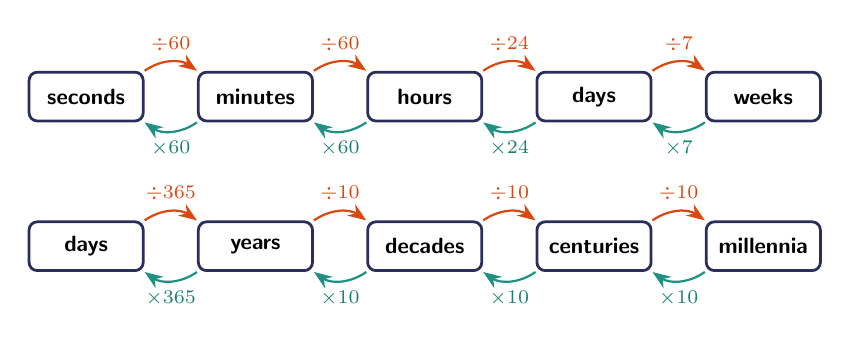
\begin{tikzpicture}[box/.style={draw=ttdark, fill=white, rounded corners=3pt, line width=1pt, minimum width=1.45cm, minimum height=0.62cm, font=\footnotesize\bfseries},
  up/.style={-{Stealth}, ttaccent, thick}, lab/.style={font=\scriptsize, text=ttaccent}]
\foreach \n/\x in {seconds/0, minutes/2.15, hours/4.3, days/6.45, weeks/8.6} \node[box] (\n) at (\x,0) {\n};
\foreach \a/\b/\k in {seconds/minutes/60, minutes/hours/60, hours/days/24, days/weeks/7}{
  \draw[up] ($(\a.north east)+(0,0)$) to[bend left=35] node[above, lab]{$\div\k$} ($(\b.north west)$);
  \draw[up, ttglow!80!black] ($(\b.south west)$) to[bend left=35] node[below, lab, text=ttglow!70!black]{$\times\k$} ($(\a.south east)$);}
\foreach \n/\x in {days/0, years/2.15, decades/4.3, centuries/6.45, millennia/8.6} \node[box] (\n2) at (\x,-1.9) {\n};
\foreach \a/\b/\k in {days/years/365, years/decades/10, decades/centuries/10, centuries/millennia/10}{
  \draw[up] ($(\a2.north east)$) to[bend left=35] node[above, lab]{$\div\k$} ($(\b2.north west)$);
  \draw[up, ttglow!80!black] ($(\b2.south west)$) to[bend left=35] node[below, lab, text=ttglow!70!black]{$\times\k$} ($(\a2.south east)$);}
\end{tikzpicture}\end{minipage}\hfill\begin{minipage}[c]{0.32\linewidth}\factbox{5.4cm}{\textbf{Leap years}\\ A normal year has 365 days. A \textbf{leap year} has 366 (it has 29 February).\\[3pt]Leap years are divisible by 4 \ldots\ \emph{except} century years (like 1900), which must be divisible by 400.}\end{minipage}\par\medskip
{\small\textbf{1.}\ Convert:\par\smallskip\begin{tabular}{rclp{1.6cm}p{0.6cm}rcll}3 weeks & = & \rule{1.6cm}{0.4pt} & days && 4 centuries & = & \rule{1.6cm}{0.4pt} & decades\\[4pt]
2 days & = & \rule{1.6cm}{0.4pt} & hours && 2 millennia & = & \rule{1.6cm}{0.4pt} & centuries\\[4pt]
180 minutes & = & \rule{1.6cm}{0.4pt} & hours && 7200 seconds & = & \rule{1.6cm}{0.4pt} & hours\\[4pt]
5 decades & = & \rule{1.6cm}{0.4pt} & years && 3 days & = & \rule{1.6cm}{0.4pt} & minutes\\[4pt]\end{tabular}}\par\medskip
{\small \begin{enumerate}[label=\textbf{\arabic*.}, leftmargin=*, itemsep=5pt, topsep=4pt, start=2]
\item Write each dial reading in a more sensible way.\par\smallskip\begin{tabular}{@{}ll}\dial{FORWARD}{72}{HOURS} & = \rule{3.5cm}{0.4pt} days\\[5pt]\dial{FORWARD}{420}{DAYS} & = \rule{3.5cm}{0.4pt} weeks\\[5pt]\dial{BACK}{1000}{HOURS} & = \rule{1.5cm}{0.4pt} days and \rule{1.5cm}{0.4pt} hours\\[5pt]\dial{BACK}{1000000}{SECONDS} & \textbf{Challenge:} = \rule{0.8cm}{0.4pt} d \rule{0.8cm}{0.4pt} h \rule{0.8cm}{0.4pt} min \rule{0.8cm}{0.4pt} s\end{tabular}
\item Dr Chrono lands on \textbf{29 February}. Which of these years could it be? Circle them: \quad 2028 \quad 2030 \quad 2100 \quad 2400
\item Put these jumps in order from \textbf{shortest} to \textbf{longest}:\par\smallskip\dial{JUMP}{1000}{HOURS}\ \ \dial{JUMP}{6}{WEEKS}\ \ \dial{JUMP}{50000}{MINUTES}\par\smallskip\dial{JUMP}{1000000}{SECONDS}\ \ \dial{JUMP}{0.1}{YEARS}\par\vspace{6pt}\rule{\linewidth}{0.4pt}
\end{enumerate}}
\clearpage
\banner{Part C \quad Timeline jumps --- giant leaps}\par\smallskip
\noindent\begin{minipage}[c]{0.44\linewidth}{\small For really big jumps, Dr Chrono uses timelines. Years \textbf{BC} count \emph{backwards}: 2560 BC is further in the past than 776 BC. Years \textbf{AD} count forwards from AD 1.}\end{minipage}\hfill\begin{minipage}[c]{0.54\linewidth}\factbox{9.3cm}{\textbf{Watch out: there is no year 0!} 1 BC is followed straight away by AD 1.\\[2pt]\emph{Example:} from 776 BC to AD 43.\\ 776 BC $\to$ 1 BC is 775 years; 1 BC $\to$ AD 1 is 1 year; AD 1 $\to$ AD 43 is 42 years.\\Total $= 775 + 1 + 42 = \mathbf{818}$ years. \quad Shortcut: $776 + 43 - 1$.}\end{minipage}\par\medskip
{\small\bfseries The big timeline: 3000 BC to AD 3000} \hfill {\scriptsize small marks every century}\par\vspace{18pt}
\begin{center}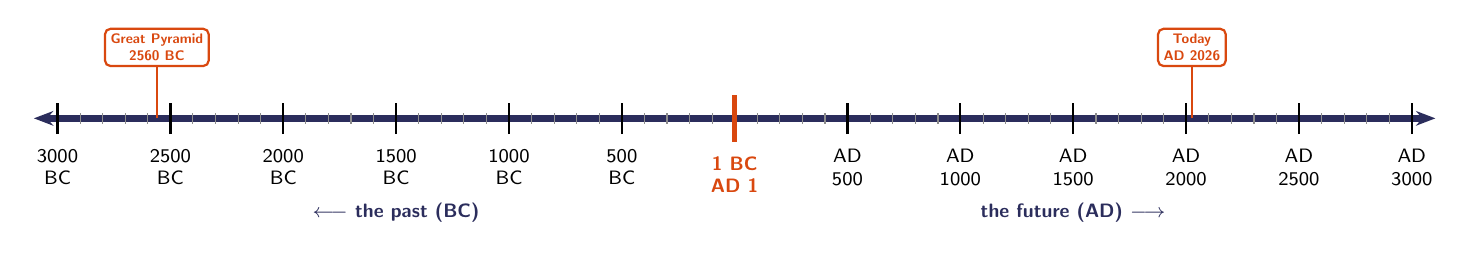
\begin{tikzpicture}
\draw[line width=2.4pt, ttdark, {Stealth[length=7pt]}-{Stealth[length=7pt]}] (-0.3,0) -- (17.50,0);
\draw[black!45] (0.000,-0.07) -- (0.000,0.07);
\draw[black!45] (0.287,-0.07) -- (0.287,0.07);
\draw[black!45] (0.573,-0.07) -- (0.573,0.07);
\draw[black!45] (0.860,-0.07) -- (0.860,0.07);
\draw[black!45] (1.147,-0.07) -- (1.147,0.07);
\draw[black!45] (1.434,-0.07) -- (1.434,0.07);
\draw[black!45] (1.720,-0.07) -- (1.720,0.07);
\draw[black!45] (2.007,-0.07) -- (2.007,0.07);
\draw[black!45] (2.294,-0.07) -- (2.294,0.07);
\draw[black!45] (2.580,-0.07) -- (2.580,0.07);
\draw[black!45] (2.867,-0.07) -- (2.867,0.07);
\draw[black!45] (3.154,-0.07) -- (3.154,0.07);
\draw[black!45] (3.441,-0.07) -- (3.441,0.07);
\draw[black!45] (3.727,-0.07) -- (3.727,0.07);
\draw[black!45] (4.014,-0.07) -- (4.014,0.07);
\draw[black!45] (4.301,-0.07) -- (4.301,0.07);
\draw[black!45] (4.587,-0.07) -- (4.587,0.07);
\draw[black!45] (4.874,-0.07) -- (4.874,0.07);
\draw[black!45] (5.161,-0.07) -- (5.161,0.07);
\draw[black!45] (5.448,-0.07) -- (5.448,0.07);
\draw[black!45] (5.734,-0.07) -- (5.734,0.07);
\draw[black!45] (6.021,-0.07) -- (6.021,0.07);
\draw[black!45] (6.308,-0.07) -- (6.308,0.07);
\draw[black!45] (6.594,-0.07) -- (6.594,0.07);
\draw[black!45] (6.881,-0.07) -- (6.881,0.07);
\draw[black!45] (7.168,-0.07) -- (7.168,0.07);
\draw[black!45] (7.455,-0.07) -- (7.455,0.07);
\draw[black!45] (7.741,-0.07) -- (7.741,0.07);
\draw[black!45] (8.028,-0.07) -- (8.028,0.07);
\draw[black!45] (8.315,-0.07) -- (8.315,0.07);
\draw[black!45] (8.601,-0.07) -- (8.601,0.07);
\draw[black!45] (8.888,-0.07) -- (8.888,0.07);
\draw[black!45] (9.175,-0.07) -- (9.175,0.07);
\draw[black!45] (9.462,-0.07) -- (9.462,0.07);
\draw[black!45] (9.748,-0.07) -- (9.748,0.07);
\draw[black!45] (10.035,-0.07) -- (10.035,0.07);
\draw[black!45] (10.322,-0.07) -- (10.322,0.07);
\draw[black!45] (10.608,-0.07) -- (10.608,0.07);
\draw[black!45] (10.895,-0.07) -- (10.895,0.07);
\draw[black!45] (11.182,-0.07) -- (11.182,0.07);
\draw[black!45] (11.469,-0.07) -- (11.469,0.07);
\draw[black!45] (11.755,-0.07) -- (11.755,0.07);
\draw[black!45] (12.042,-0.07) -- (12.042,0.07);
\draw[black!45] (12.329,-0.07) -- (12.329,0.07);
\draw[black!45] (12.615,-0.07) -- (12.615,0.07);
\draw[black!45] (12.902,-0.07) -- (12.902,0.07);
\draw[black!45] (13.189,-0.07) -- (13.189,0.07);
\draw[black!45] (13.476,-0.07) -- (13.476,0.07);
\draw[black!45] (13.762,-0.07) -- (13.762,0.07);
\draw[black!45] (14.049,-0.07) -- (14.049,0.07);
\draw[black!45] (14.336,-0.07) -- (14.336,0.07);
\draw[black!45] (14.622,-0.07) -- (14.622,0.07);
\draw[black!45] (14.909,-0.07) -- (14.909,0.07);
\draw[black!45] (15.196,-0.07) -- (15.196,0.07);
\draw[black!45] (15.483,-0.07) -- (15.483,0.07);
\draw[black!45] (15.769,-0.07) -- (15.769,0.07);
\draw[black!45] (16.056,-0.07) -- (16.056,0.07);
\draw[black!45] (16.343,-0.07) -- (16.343,0.07);
\draw[black!45] (16.629,-0.07) -- (16.629,0.07);
\draw[black!45] (16.916,-0.07) -- (16.916,0.07);
\draw[thick] (0.000,-0.2) -- (0.000,0.2);
\node[font=\scriptsize, below=2pt, align=center] at (0.000,-0.2) {3000\\BC};
\draw[thick] (1.434,-0.2) -- (1.434,0.2);
\node[font=\scriptsize, below=2pt, align=center] at (1.434,-0.2) {2500\\BC};
\draw[thick] (2.867,-0.2) -- (2.867,0.2);
\node[font=\scriptsize, below=2pt, align=center] at (2.867,-0.2) {2000\\BC};
\draw[thick] (4.301,-0.2) -- (4.301,0.2);
\node[font=\scriptsize, below=2pt, align=center] at (4.301,-0.2) {1500\\BC};
\draw[thick] (5.734,-0.2) -- (5.734,0.2);
\node[font=\scriptsize, below=2pt, align=center] at (5.734,-0.2) {1000\\BC};
\draw[thick] (7.168,-0.2) -- (7.168,0.2);
\node[font=\scriptsize, below=2pt, align=center] at (7.168,-0.2) {500\\BC};
\draw[ultra thick, ttaccent] (8.600,-0.3) -- (8.600,0.3);
\node[font=\scriptsize\bfseries, below=2pt, align=center, text=ttaccent] at (8.600,-0.3) {1 BC\\AD 1};
\draw[thick] (10.032,-0.2) -- (10.032,0.2);
\node[font=\scriptsize, below=2pt, align=center] at (10.032,-0.2) {AD\\500};
\draw[thick] (11.466,-0.2) -- (11.466,0.2);
\node[font=\scriptsize, below=2pt, align=center] at (11.466,-0.2) {AD\\1000};
\draw[thick] (12.899,-0.2) -- (12.899,0.2);
\node[font=\scriptsize, below=2pt, align=center] at (12.899,-0.2) {AD\\1500};
\draw[thick] (14.333,-0.2) -- (14.333,0.2);
\node[font=\scriptsize, below=2pt, align=center] at (14.333,-0.2) {AD\\2000};
\draw[thick] (15.766,-0.2) -- (15.766,0.2);
\node[font=\scriptsize, below=2pt, align=center] at (15.766,-0.2) {AD\\2500};
\draw[thick] (17.200,-0.2) -- (17.200,0.2);
\node[font=\scriptsize, below=2pt, align=center] at (17.200,-0.2) {AD\\3000};
\node[font=\scriptsize\bfseries, text=ttdark] at (4.298,-1.2) {$\longleftarrow$ the past (BC)};
\node[font=\scriptsize\bfseries, text=ttdark] at (12.899,-1.2) {the future (AD) $\longrightarrow$};
\draw[ttaccent, thick] (1.262,0) -- (1.262,0.7);
\node[flag, above] at (1.262,0.65) {Great Pyramid\\2560 BC};
\draw[ttaccent, thick] (14.407,0) -- (14.407,0.7);
\node[flag, above] at (14.407,0.65) {Today\\AD 2026};
\end{tikzpicture}\end{center}\vspace{6pt}
{\small\bfseries The zoomed timeline: AD 1000 to AD 2100}\par\vspace{18pt}
\begin{center}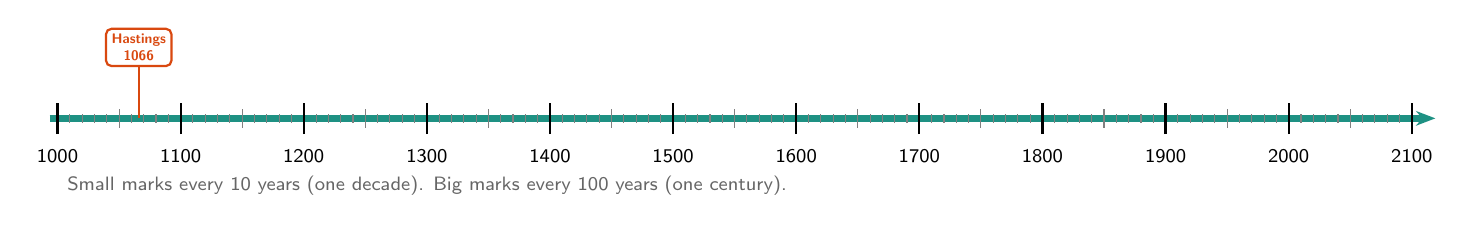
\begin{tikzpicture}
\draw[line width=2.4pt, ttglow!80!black, -{Stealth[length=7pt]}] (-0.1,0) -- (17.50,0);
\draw[thick] (0.000,-0.20) -- (0.000,0.20);
\node[font=\scriptsize, below=2pt] at (0.000,-0.2) {1000};
\draw[black!50] (0.156,-0.06) -- (0.156,0.06);
\draw[black!50] (0.313,-0.06) -- (0.313,0.06);
\draw[black!50] (0.469,-0.06) -- (0.469,0.06);
\draw[black!50] (0.625,-0.06) -- (0.625,0.06);
\draw[black!50] (0.782,-0.12) -- (0.782,0.12);
\draw[black!50] (0.938,-0.06) -- (0.938,0.06);
\draw[black!50] (1.095,-0.06) -- (1.095,0.06);
\draw[black!50] (1.251,-0.06) -- (1.251,0.06);
\draw[black!50] (1.407,-0.06) -- (1.407,0.06);
\draw[thick] (1.564,-0.20) -- (1.564,0.20);
\node[font=\scriptsize, below=2pt] at (1.564,-0.2) {1100};
\draw[black!50] (1.720,-0.06) -- (1.720,0.06);
\draw[black!50] (1.876,-0.06) -- (1.876,0.06);
\draw[black!50] (2.033,-0.06) -- (2.033,0.06);
\draw[black!50] (2.189,-0.06) -- (2.189,0.06);
\draw[black!50] (2.345,-0.12) -- (2.345,0.12);
\draw[black!50] (2.502,-0.06) -- (2.502,0.06);
\draw[black!50] (2.658,-0.06) -- (2.658,0.06);
\draw[black!50] (2.815,-0.06) -- (2.815,0.06);
\draw[black!50] (2.971,-0.06) -- (2.971,0.06);
\draw[thick] (3.127,-0.20) -- (3.127,0.20);
\node[font=\scriptsize, below=2pt] at (3.127,-0.2) {1200};
\draw[black!50] (3.284,-0.06) -- (3.284,0.06);
\draw[black!50] (3.440,-0.06) -- (3.440,0.06);
\draw[black!50] (3.596,-0.06) -- (3.596,0.06);
\draw[black!50] (3.753,-0.06) -- (3.753,0.06);
\draw[black!50] (3.909,-0.12) -- (3.909,0.12);
\draw[black!50] (4.065,-0.06) -- (4.065,0.06);
\draw[black!50] (4.222,-0.06) -- (4.222,0.06);
\draw[black!50] (4.378,-0.06) -- (4.378,0.06);
\draw[black!50] (4.535,-0.06) -- (4.535,0.06);
\draw[thick] (4.691,-0.20) -- (4.691,0.20);
\node[font=\scriptsize, below=2pt] at (4.691,-0.2) {1300};
\draw[black!50] (4.847,-0.06) -- (4.847,0.06);
\draw[black!50] (5.004,-0.06) -- (5.004,0.06);
\draw[black!50] (5.160,-0.06) -- (5.160,0.06);
\draw[black!50] (5.316,-0.06) -- (5.316,0.06);
\draw[black!50] (5.473,-0.12) -- (5.473,0.12);
\draw[black!50] (5.629,-0.06) -- (5.629,0.06);
\draw[black!50] (5.785,-0.06) -- (5.785,0.06);
\draw[black!50] (5.942,-0.06) -- (5.942,0.06);
\draw[black!50] (6.098,-0.06) -- (6.098,0.06);
\draw[thick] (6.255,-0.20) -- (6.255,0.20);
\node[font=\scriptsize, below=2pt] at (6.255,-0.2) {1400};
\draw[black!50] (6.411,-0.06) -- (6.411,0.06);
\draw[black!50] (6.567,-0.06) -- (6.567,0.06);
\draw[black!50] (6.724,-0.06) -- (6.724,0.06);
\draw[black!50] (6.880,-0.06) -- (6.880,0.06);
\draw[black!50] (7.036,-0.12) -- (7.036,0.12);
\draw[black!50] (7.193,-0.06) -- (7.193,0.06);
\draw[black!50] (7.349,-0.06) -- (7.349,0.06);
\draw[black!50] (7.505,-0.06) -- (7.505,0.06);
\draw[black!50] (7.662,-0.06) -- (7.662,0.06);
\draw[thick] (7.818,-0.20) -- (7.818,0.20);
\node[font=\scriptsize, below=2pt] at (7.818,-0.2) {1500};
\draw[black!50] (7.975,-0.06) -- (7.975,0.06);
\draw[black!50] (8.131,-0.06) -- (8.131,0.06);
\draw[black!50] (8.287,-0.06) -- (8.287,0.06);
\draw[black!50] (8.444,-0.06) -- (8.444,0.06);
\draw[black!50] (8.600,-0.12) -- (8.600,0.12);
\draw[black!50] (8.756,-0.06) -- (8.756,0.06);
\draw[black!50] (8.913,-0.06) -- (8.913,0.06);
\draw[black!50] (9.069,-0.06) -- (9.069,0.06);
\draw[black!50] (9.225,-0.06) -- (9.225,0.06);
\draw[thick] (9.382,-0.20) -- (9.382,0.20);
\node[font=\scriptsize, below=2pt] at (9.382,-0.2) {1600};
\draw[black!50] (9.538,-0.06) -- (9.538,0.06);
\draw[black!50] (9.695,-0.06) -- (9.695,0.06);
\draw[black!50] (9.851,-0.06) -- (9.851,0.06);
\draw[black!50] (10.007,-0.06) -- (10.007,0.06);
\draw[black!50] (10.164,-0.12) -- (10.164,0.12);
\draw[black!50] (10.320,-0.06) -- (10.320,0.06);
\draw[black!50] (10.476,-0.06) -- (10.476,0.06);
\draw[black!50] (10.633,-0.06) -- (10.633,0.06);
\draw[black!50] (10.789,-0.06) -- (10.789,0.06);
\draw[thick] (10.945,-0.20) -- (10.945,0.20);
\node[font=\scriptsize, below=2pt] at (10.945,-0.2) {1700};
\draw[black!50] (11.102,-0.06) -- (11.102,0.06);
\draw[black!50] (11.258,-0.06) -- (11.258,0.06);
\draw[black!50] (11.415,-0.06) -- (11.415,0.06);
\draw[black!50] (11.571,-0.06) -- (11.571,0.06);
\draw[black!50] (11.727,-0.12) -- (11.727,0.12);
\draw[black!50] (11.884,-0.06) -- (11.884,0.06);
\draw[black!50] (12.040,-0.06) -- (12.040,0.06);
\draw[black!50] (12.196,-0.06) -- (12.196,0.06);
\draw[black!50] (12.353,-0.06) -- (12.353,0.06);
\draw[thick] (12.509,-0.20) -- (12.509,0.20);
\node[font=\scriptsize, below=2pt] at (12.509,-0.2) {1800};
\draw[black!50] (12.665,-0.06) -- (12.665,0.06);
\draw[black!50] (12.822,-0.06) -- (12.822,0.06);
\draw[black!50] (12.978,-0.06) -- (12.978,0.06);
\draw[black!50] (13.135,-0.06) -- (13.135,0.06);
\draw[black!50] (13.291,-0.12) -- (13.291,0.12);
\draw[black!50] (13.447,-0.06) -- (13.447,0.06);
\draw[black!50] (13.604,-0.06) -- (13.604,0.06);
\draw[black!50] (13.760,-0.06) -- (13.760,0.06);
\draw[black!50] (13.916,-0.06) -- (13.916,0.06);
\draw[thick] (14.073,-0.20) -- (14.073,0.20);
\node[font=\scriptsize, below=2pt] at (14.073,-0.2) {1900};
\draw[black!50] (14.229,-0.06) -- (14.229,0.06);
\draw[black!50] (14.385,-0.06) -- (14.385,0.06);
\draw[black!50] (14.542,-0.06) -- (14.542,0.06);
\draw[black!50] (14.698,-0.06) -- (14.698,0.06);
\draw[black!50] (14.855,-0.12) -- (14.855,0.12);
\draw[black!50] (15.011,-0.06) -- (15.011,0.06);
\draw[black!50] (15.167,-0.06) -- (15.167,0.06);
\draw[black!50] (15.324,-0.06) -- (15.324,0.06);
\draw[black!50] (15.480,-0.06) -- (15.480,0.06);
\draw[thick] (15.636,-0.20) -- (15.636,0.20);
\node[font=\scriptsize, below=2pt] at (15.636,-0.2) {2000};
\draw[black!50] (15.793,-0.06) -- (15.793,0.06);
\draw[black!50] (15.949,-0.06) -- (15.949,0.06);
\draw[black!50] (16.105,-0.06) -- (16.105,0.06);
\draw[black!50] (16.262,-0.06) -- (16.262,0.06);
\draw[black!50] (16.418,-0.12) -- (16.418,0.12);
\draw[black!50] (16.575,-0.06) -- (16.575,0.06);
\draw[black!50] (16.731,-0.06) -- (16.731,0.06);
\draw[black!50] (16.887,-0.06) -- (16.887,0.06);
\draw[black!50] (17.044,-0.06) -- (17.044,0.06);
\draw[thick] (17.200,-0.20) -- (17.200,0.20);
\node[font=\scriptsize, below=2pt] at (17.200,-0.2) {2100};
\node[font=\scriptsize, text=black!60, anchor=west] at (0,-0.85) {Small marks every 10 years (one decade). Big marks every 100 years (one century).};
\draw[ttaccent, thick] (1.032,0) -- (1.032,0.7);
\node[flag, above] at (1.032,0.65) {Hastings\\1066};
\end{tikzpicture}\end{center}
{\small \begin{enumerate}[label=\textbf{\arabic*.}, leftmargin=*, itemsep=5pt, topsep=4pt, start=1]
\item Mark these on the big timeline with a cross and a label: \quad Tutankhamun dies \textbf{1323 BC} \quad First Olympic Games \textbf{776 BC} \quad Romans invade Britain \textbf{AD 43} \quad Battle of Hastings \textbf{AD 1066}
\item How many years ago (from 2026) was \ldots\par\smallskip\begin{tabular}{@{}l@{\ }l@{\qquad}l@{\ }l}(a) the Battle of Hastings? & \aline & (b) the Roman invasion? & \aline\\[5pt](c) the first Olympic Games? & \aline & (d) the Great Pyramid? & \aline\end{tabular}
\item Write your answer to 2(a) in centuries and decades: \lline
\item Where (when!) does the machine land? Mark these on the big timeline too.\par\smallskip\begin{tabular}{@{}l@{\ }l}from 2026: \dial{BACK}{3}{MILLENNIA} & lands in \lline\\[5pt]from 2026: \dial{FORWARD}{5}{CENTURIES} & lands in \lline\\[5pt]from 2026: \dial{BACK}{25}{CENTURIES} & lands in \lline\end{tabular}
\item \textbf{Zoom in:} mark these on the zoomed timeline: \quad Magna Carta \textbf{1215} \quad Great Fire of London \textbf{1666} \quad Moon landing \textbf{1969} \quad Today \textbf{2026}
\item How many years from (a) Magna Carta to the Great Fire? \aline\quad (b) the Moon landing to today? \aline
\item Is the Great Fire of London closer in time to the Battle of Hastings, or to today? Show how you know.\par\vspace{4pt}\rule{\linewidth}{0.4pt}
\end{enumerate}}
\clearpage
\banner{Part D \quad Mission log --- getting home}\par\smallskip
{\small Dr Chrono sets off from \textbf{AD 2026} and makes four jumps. Her battery starts at \textbf{100\%}, and every \textbf{century} of travel (forwards or backwards) uses \textbf{2\%} of the battery.}\par\medskip
\begin{center}{\small\begin{tabular}{c|c|p{3.2cm}|p{3.2cm}}\textbf{Jump} & \textbf{Dial} & \textbf{From} & \textbf{Lands in}\\\hline
1 & \dial{BACK}{3}{CENTURIES} & AD 2026 & \\[3pt]\hline
2 & \dial{FORWARD}{25}{YEARS} &  & \\[3pt]\hline
3 & \dial{BACK}{2}{MILLENNIA} &  & \\[3pt]\hline
4 & \dial{FORWARD}{1500}{YEARS} &  & \\[3pt]\hline\end{tabular}}\end{center}
{\small \begin{enumerate}[label=\textbf{\arabic*.}, leftmargin=*, itemsep=5pt, topsep=4pt, start=1]
\item What single jump would take Dr Chrono straight home to AD 2026? \par\smallskip FORWARD or BACK? \aline\quad How many years? \aline
\item How many years did she travel in jumps 1--4 altogether? \aline\quad How many centuries is that? \aline
\item How much battery has she used so far? \aline\quad How much is left? \aline
\item Does she have enough battery to make the jump home? Show your working.\par\vspace{4pt}\rule{\linewidth}{0.4pt}
\item \textbf{Design a mission:} plan three jumps that visit the Great Pyramid, the Battle of Hastings and the Moon landing, then come home. Write your dial settings and work out the battery used.\par\medskip\begin{center}\begin{tabular}{c|p{3.4cm}|p{3.4cm}|p{3.4cm}}\textbf{Jump} & \textbf{Dial setting} & \textbf{Lands in} & \textbf{Battery used}\\\hline1 & & & \\[10pt]\hline 2 & & & \\[10pt]\hline 3 & & & \\[10pt]\hline Home & & & \\[10pt]\hline\multicolumn{3}{r|}{\textbf{Total battery used}} & \\[10pt]\hline\end{tabular}\end{center}
\end{enumerate}}
\clearpage\enlargethispage{3\baselineskip}\begin{center}{\LARGE\bfseries Answers}\end{center}\vspace{-6pt}
\banner{Part A \quad Calendar hops --- small jumps}\par\smallskip
{\small \begin{enumerate}[label=\textbf{\arabic*.}, leftmargin=*, itemsep=5pt, topsep=4pt, start=1]
\item \dial{FORWARD}{1}{WEEK} \quad Day and date: \lline\par\ans{Saturday 7 November 2026}
\item \dial{FORWARD}{10}{DAYS} \quad Day and date: \lline\par\ans{Tuesday 10 November 2026}
\item \dial{BACK}{2}{WEEKS} \quad Day and date: \lline\par\ans{Saturday 17 October 2026}
\item \dial{FORWARD}{3 WEEKS}{+ 2 DAYS} \quad Day and date: \lline\par\ans{Monday 23 November 2026}
\item \dial{BACK}{45}{DAYS} \quad Day and date: \lline\par\ans{Wednesday 16 September 2026}
\item \dial{FORWARD}{100}{HOURS} \quad Day, date \emph{and time}: \lline\par\ans{Wednesday 4 November 2026 at 14:00 (100 hours = 4 days 4 hours)}
\item Dr Chrono wants to watch the fireworks on Bonfire Night (5 November) and then jump to Christmas Day (25 December). How many days forward is that? \aline\ \ Write it in weeks and days: \aline\par\ans{50 days = 7 weeks 1 day}
\item The dial gets stuck so it can only jump in \textbf{whole weeks}. Starting from today, can Dr Chrono land exactly on Christmas Day? Explain, and say which two dates nearest Christmas it \emph{can} reach.\par\vspace{4pt}\rule{\linewidth}{0.4pt}\par\ans{No. 31 Oct to 25 Dec is 55 days, not a multiple of 7. Whole weeks from a Saturday always land on a Saturday: Sat 19 Dec (7 weeks) or Sat 26 Dec (8 weeks).}
\item \textbf{Spooky landing:} Dr Chrono's machine always breaks down on a Friday the 13th. Which date on these calendars should she avoid? \lline\par\ans{Friday 13 November 2026}
\end{enumerate}}
\banner{Part B \quad Conversion station --- medium jumps}\par\smallskip
{\small\textbf{1.}\ Convert:\par\smallskip\begin{tabular}{rclp{1.6cm}p{0.6cm}rcll}3 weeks & = & \ans{21} & days && 4 centuries & = & \ans{40} & decades\\[4pt]
2 days & = & \ans{48} & hours && 2 millennia & = & \ans{20} & centuries\\[4pt]
180 minutes & = & \ans{3} & hours && 7200 seconds & = & \ans{2} & hours\\[4pt]
5 decades & = & \ans{50} & years && 3 days & = & \ans{4320} & minutes\\[4pt]\end{tabular}}\par\medskip
{\small \begin{enumerate}[label=\textbf{\arabic*.}, leftmargin=*, itemsep=5pt, topsep=4pt, start=2]
\item Write each dial reading in a more sensible way.\par\smallskip\begin{tabular}{@{}ll}\dial{FORWARD}{72}{HOURS} & = \rule{3.5cm}{0.4pt} days\\[5pt]\dial{FORWARD}{420}{DAYS} & = \rule{3.5cm}{0.4pt} weeks\\[5pt]\dial{BACK}{1000}{HOURS} & = \rule{1.5cm}{0.4pt} days and \rule{1.5cm}{0.4pt} hours\\[5pt]\dial{BACK}{1000000}{SECONDS} & \textbf{Challenge:} = \rule{0.8cm}{0.4pt} d \rule{0.8cm}{0.4pt} h \rule{0.8cm}{0.4pt} min \rule{0.8cm}{0.4pt} s\end{tabular}\par\ans{3 days;\quad 60 weeks;\quad 41 days 16 hours;\quad 11 d 13 h 46 min 40 s}
\item Dr Chrono lands on \textbf{29 February}. Which of these years could it be? Circle them: \quad 2028 \quad 2030 \quad 2100 \quad 2400\par\ans{2028 and 2400 (2030 is not divisible by 4; 2100 is a century year not divisible by 400)}
\item Put these jumps in order from \textbf{shortest} to \textbf{longest}:\par\smallskip\dial{JUMP}{1000}{HOURS}\ \ \dial{JUMP}{6}{WEEKS}\ \ \dial{JUMP}{50000}{MINUTES}\par\smallskip\dial{JUMP}{1000000}{SECONDS}\ \ \dial{JUMP}{0.1}{YEARS}\par\vspace{6pt}\rule{\linewidth}{0.4pt}\par\ans{1\,000\,000 s ($\approx$ 11.6 days) $<$ 50\,000 min ($\approx$ 34.7 days) $<$ 0.1 years (36.5 days) $<$ 1000 hours ($\approx$ 41.7 days) $<$ 6 weeks (42 days)}
\end{enumerate}}
\clearpage
\banner{Part C \quad Timeline jumps --- giant leaps}\par\smallskip
{\small\bfseries The big timeline: 3000 BC to AD 3000} \hfill {\scriptsize small marks every century}\par\vspace{18pt}
\begin{center}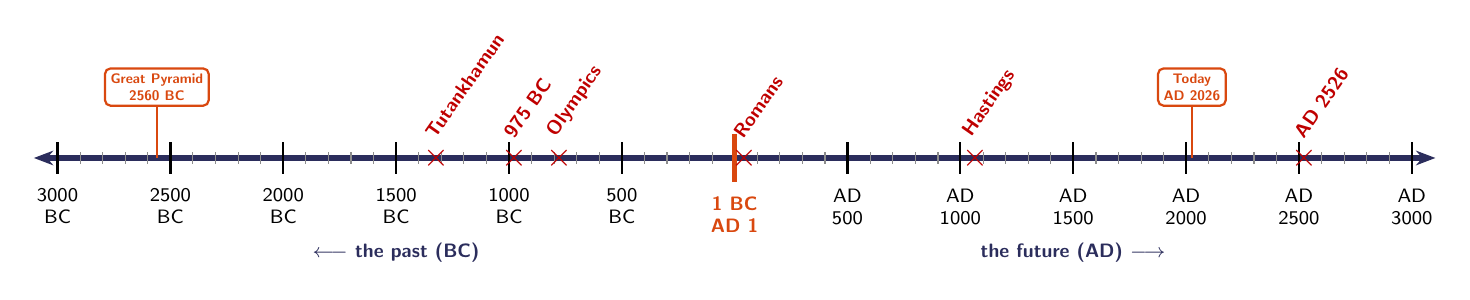
\begin{tikzpicture}
\draw[line width=2.4pt, ttdark, {Stealth[length=7pt]}-{Stealth[length=7pt]}] (-0.3,0) -- (17.50,0);
\draw[black!45] (0.000,-0.07) -- (0.000,0.07);
\draw[black!45] (0.287,-0.07) -- (0.287,0.07);
\draw[black!45] (0.573,-0.07) -- (0.573,0.07);
\draw[black!45] (0.860,-0.07) -- (0.860,0.07);
\draw[black!45] (1.147,-0.07) -- (1.147,0.07);
\draw[black!45] (1.434,-0.07) -- (1.434,0.07);
\draw[black!45] (1.720,-0.07) -- (1.720,0.07);
\draw[black!45] (2.007,-0.07) -- (2.007,0.07);
\draw[black!45] (2.294,-0.07) -- (2.294,0.07);
\draw[black!45] (2.580,-0.07) -- (2.580,0.07);
\draw[black!45] (2.867,-0.07) -- (2.867,0.07);
\draw[black!45] (3.154,-0.07) -- (3.154,0.07);
\draw[black!45] (3.441,-0.07) -- (3.441,0.07);
\draw[black!45] (3.727,-0.07) -- (3.727,0.07);
\draw[black!45] (4.014,-0.07) -- (4.014,0.07);
\draw[black!45] (4.301,-0.07) -- (4.301,0.07);
\draw[black!45] (4.587,-0.07) -- (4.587,0.07);
\draw[black!45] (4.874,-0.07) -- (4.874,0.07);
\draw[black!45] (5.161,-0.07) -- (5.161,0.07);
\draw[black!45] (5.448,-0.07) -- (5.448,0.07);
\draw[black!45] (5.734,-0.07) -- (5.734,0.07);
\draw[black!45] (6.021,-0.07) -- (6.021,0.07);
\draw[black!45] (6.308,-0.07) -- (6.308,0.07);
\draw[black!45] (6.594,-0.07) -- (6.594,0.07);
\draw[black!45] (6.881,-0.07) -- (6.881,0.07);
\draw[black!45] (7.168,-0.07) -- (7.168,0.07);
\draw[black!45] (7.455,-0.07) -- (7.455,0.07);
\draw[black!45] (7.741,-0.07) -- (7.741,0.07);
\draw[black!45] (8.028,-0.07) -- (8.028,0.07);
\draw[black!45] (8.315,-0.07) -- (8.315,0.07);
\draw[black!45] (8.601,-0.07) -- (8.601,0.07);
\draw[black!45] (8.888,-0.07) -- (8.888,0.07);
\draw[black!45] (9.175,-0.07) -- (9.175,0.07);
\draw[black!45] (9.462,-0.07) -- (9.462,0.07);
\draw[black!45] (9.748,-0.07) -- (9.748,0.07);
\draw[black!45] (10.035,-0.07) -- (10.035,0.07);
\draw[black!45] (10.322,-0.07) -- (10.322,0.07);
\draw[black!45] (10.608,-0.07) -- (10.608,0.07);
\draw[black!45] (10.895,-0.07) -- (10.895,0.07);
\draw[black!45] (11.182,-0.07) -- (11.182,0.07);
\draw[black!45] (11.469,-0.07) -- (11.469,0.07);
\draw[black!45] (11.755,-0.07) -- (11.755,0.07);
\draw[black!45] (12.042,-0.07) -- (12.042,0.07);
\draw[black!45] (12.329,-0.07) -- (12.329,0.07);
\draw[black!45] (12.615,-0.07) -- (12.615,0.07);
\draw[black!45] (12.902,-0.07) -- (12.902,0.07);
\draw[black!45] (13.189,-0.07) -- (13.189,0.07);
\draw[black!45] (13.476,-0.07) -- (13.476,0.07);
\draw[black!45] (13.762,-0.07) -- (13.762,0.07);
\draw[black!45] (14.049,-0.07) -- (14.049,0.07);
\draw[black!45] (14.336,-0.07) -- (14.336,0.07);
\draw[black!45] (14.622,-0.07) -- (14.622,0.07);
\draw[black!45] (14.909,-0.07) -- (14.909,0.07);
\draw[black!45] (15.196,-0.07) -- (15.196,0.07);
\draw[black!45] (15.483,-0.07) -- (15.483,0.07);
\draw[black!45] (15.769,-0.07) -- (15.769,0.07);
\draw[black!45] (16.056,-0.07) -- (16.056,0.07);
\draw[black!45] (16.343,-0.07) -- (16.343,0.07);
\draw[black!45] (16.629,-0.07) -- (16.629,0.07);
\draw[black!45] (16.916,-0.07) -- (16.916,0.07);
\draw[thick] (0.000,-0.2) -- (0.000,0.2);
\node[font=\scriptsize, below=2pt, align=center] at (0.000,-0.2) {3000\\BC};
\draw[thick] (1.434,-0.2) -- (1.434,0.2);
\node[font=\scriptsize, below=2pt, align=center] at (1.434,-0.2) {2500\\BC};
\draw[thick] (2.867,-0.2) -- (2.867,0.2);
\node[font=\scriptsize, below=2pt, align=center] at (2.867,-0.2) {2000\\BC};
\draw[thick] (4.301,-0.2) -- (4.301,0.2);
\node[font=\scriptsize, below=2pt, align=center] at (4.301,-0.2) {1500\\BC};
\draw[thick] (5.734,-0.2) -- (5.734,0.2);
\node[font=\scriptsize, below=2pt, align=center] at (5.734,-0.2) {1000\\BC};
\draw[thick] (7.168,-0.2) -- (7.168,0.2);
\node[font=\scriptsize, below=2pt, align=center] at (7.168,-0.2) {500\\BC};
\draw[ultra thick, ttaccent] (8.600,-0.3) -- (8.600,0.3);
\node[font=\scriptsize\bfseries, below=2pt, align=center, text=ttaccent] at (8.600,-0.3) {1 BC\\AD 1};
\draw[thick] (10.032,-0.2) -- (10.032,0.2);
\node[font=\scriptsize, below=2pt, align=center] at (10.032,-0.2) {AD\\500};
\draw[thick] (11.466,-0.2) -- (11.466,0.2);
\node[font=\scriptsize, below=2pt, align=center] at (11.466,-0.2) {AD\\1000};
\draw[thick] (12.899,-0.2) -- (12.899,0.2);
\node[font=\scriptsize, below=2pt, align=center] at (12.899,-0.2) {AD\\1500};
\draw[thick] (14.333,-0.2) -- (14.333,0.2);
\node[font=\scriptsize, below=2pt, align=center] at (14.333,-0.2) {AD\\2000};
\draw[thick] (15.766,-0.2) -- (15.766,0.2);
\node[font=\scriptsize, below=2pt, align=center] at (15.766,-0.2) {AD\\2500};
\draw[thick] (17.200,-0.2) -- (17.200,0.2);
\node[font=\scriptsize, below=2pt, align=center] at (17.200,-0.2) {AD\\3000};
\node[font=\scriptsize\bfseries, text=ttdark] at (4.298,-1.2) {$\longleftarrow$ the past (BC)};
\node[font=\scriptsize\bfseries, text=ttdark] at (12.899,-1.2) {the future (AD) $\longrightarrow$};
\draw[ttaccent, thick] (1.262,0) -- (1.262,0.7);
\node[flag, above] at (1.262,0.65) {Great Pyramid\\2560 BC};
\draw[ttaccent, thick] (14.407,0) -- (14.407,0.7);
\node[flag, above] at (14.407,0.65) {Today\\AD 2026};
\node[text=red!75!black, font=\large\bfseries] at (4.808,0) {$\times$};
\node[text=red!75!black, font=\scriptsize\bfseries, rotate=55, anchor=south west, inner sep=1pt] at (4.808,0.18) {Tutankhamun};
\node[text=red!75!black, font=\large\bfseries] at (6.377,0) {$\times$};
\node[text=red!75!black, font=\scriptsize\bfseries, rotate=55, anchor=south west, inner sep=1pt] at (6.377,0.18) {Olympics};
\node[text=red!75!black, font=\large\bfseries] at (8.722,0) {$\times$};
\node[text=red!75!black, font=\scriptsize\bfseries, rotate=55, anchor=south west, inner sep=1pt] at (8.722,0.18) {Romans};
\node[text=red!75!black, font=\large\bfseries] at (11.655,0) {$\times$};
\node[text=red!75!black, font=\scriptsize\bfseries, rotate=55, anchor=south west, inner sep=1pt] at (11.655,0.18) {Hastings};
\node[text=red!75!black, font=\large\bfseries] at (5.806,0) {$\times$};
\node[text=red!75!black, font=\scriptsize\bfseries, rotate=55, anchor=south west, inner sep=1pt] at (5.806,0.18) {975 BC};
\node[text=red!75!black, font=\large\bfseries] at (15.841,0) {$\times$};
\node[text=red!75!black, font=\scriptsize\bfseries, rotate=55, anchor=south west, inner sep=1pt] at (15.841,0.18) {AD 2526};
\end{tikzpicture}\end{center}\vspace{6pt}
{\small\bfseries The zoomed timeline: AD 1000 to AD 2100}\par\vspace{18pt}
\begin{center}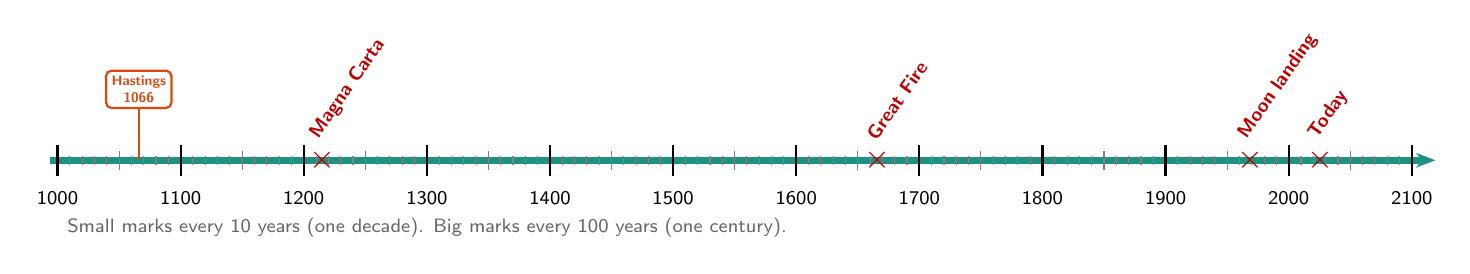
\begin{tikzpicture}
\draw[line width=2.4pt, ttglow!80!black, -{Stealth[length=7pt]}] (-0.1,0) -- (17.50,0);
\draw[thick] (0.000,-0.20) -- (0.000,0.20);
\node[font=\scriptsize, below=2pt] at (0.000,-0.2) {1000};
\draw[black!50] (0.156,-0.06) -- (0.156,0.06);
\draw[black!50] (0.313,-0.06) -- (0.313,0.06);
\draw[black!50] (0.469,-0.06) -- (0.469,0.06);
\draw[black!50] (0.625,-0.06) -- (0.625,0.06);
\draw[black!50] (0.782,-0.12) -- (0.782,0.12);
\draw[black!50] (0.938,-0.06) -- (0.938,0.06);
\draw[black!50] (1.095,-0.06) -- (1.095,0.06);
\draw[black!50] (1.251,-0.06) -- (1.251,0.06);
\draw[black!50] (1.407,-0.06) -- (1.407,0.06);
\draw[thick] (1.564,-0.20) -- (1.564,0.20);
\node[font=\scriptsize, below=2pt] at (1.564,-0.2) {1100};
\draw[black!50] (1.720,-0.06) -- (1.720,0.06);
\draw[black!50] (1.876,-0.06) -- (1.876,0.06);
\draw[black!50] (2.033,-0.06) -- (2.033,0.06);
\draw[black!50] (2.189,-0.06) -- (2.189,0.06);
\draw[black!50] (2.345,-0.12) -- (2.345,0.12);
\draw[black!50] (2.502,-0.06) -- (2.502,0.06);
\draw[black!50] (2.658,-0.06) -- (2.658,0.06);
\draw[black!50] (2.815,-0.06) -- (2.815,0.06);
\draw[black!50] (2.971,-0.06) -- (2.971,0.06);
\draw[thick] (3.127,-0.20) -- (3.127,0.20);
\node[font=\scriptsize, below=2pt] at (3.127,-0.2) {1200};
\draw[black!50] (3.284,-0.06) -- (3.284,0.06);
\draw[black!50] (3.440,-0.06) -- (3.440,0.06);
\draw[black!50] (3.596,-0.06) -- (3.596,0.06);
\draw[black!50] (3.753,-0.06) -- (3.753,0.06);
\draw[black!50] (3.909,-0.12) -- (3.909,0.12);
\draw[black!50] (4.065,-0.06) -- (4.065,0.06);
\draw[black!50] (4.222,-0.06) -- (4.222,0.06);
\draw[black!50] (4.378,-0.06) -- (4.378,0.06);
\draw[black!50] (4.535,-0.06) -- (4.535,0.06);
\draw[thick] (4.691,-0.20) -- (4.691,0.20);
\node[font=\scriptsize, below=2pt] at (4.691,-0.2) {1300};
\draw[black!50] (4.847,-0.06) -- (4.847,0.06);
\draw[black!50] (5.004,-0.06) -- (5.004,0.06);
\draw[black!50] (5.160,-0.06) -- (5.160,0.06);
\draw[black!50] (5.316,-0.06) -- (5.316,0.06);
\draw[black!50] (5.473,-0.12) -- (5.473,0.12);
\draw[black!50] (5.629,-0.06) -- (5.629,0.06);
\draw[black!50] (5.785,-0.06) -- (5.785,0.06);
\draw[black!50] (5.942,-0.06) -- (5.942,0.06);
\draw[black!50] (6.098,-0.06) -- (6.098,0.06);
\draw[thick] (6.255,-0.20) -- (6.255,0.20);
\node[font=\scriptsize, below=2pt] at (6.255,-0.2) {1400};
\draw[black!50] (6.411,-0.06) -- (6.411,0.06);
\draw[black!50] (6.567,-0.06) -- (6.567,0.06);
\draw[black!50] (6.724,-0.06) -- (6.724,0.06);
\draw[black!50] (6.880,-0.06) -- (6.880,0.06);
\draw[black!50] (7.036,-0.12) -- (7.036,0.12);
\draw[black!50] (7.193,-0.06) -- (7.193,0.06);
\draw[black!50] (7.349,-0.06) -- (7.349,0.06);
\draw[black!50] (7.505,-0.06) -- (7.505,0.06);
\draw[black!50] (7.662,-0.06) -- (7.662,0.06);
\draw[thick] (7.818,-0.20) -- (7.818,0.20);
\node[font=\scriptsize, below=2pt] at (7.818,-0.2) {1500};
\draw[black!50] (7.975,-0.06) -- (7.975,0.06);
\draw[black!50] (8.131,-0.06) -- (8.131,0.06);
\draw[black!50] (8.287,-0.06) -- (8.287,0.06);
\draw[black!50] (8.444,-0.06) -- (8.444,0.06);
\draw[black!50] (8.600,-0.12) -- (8.600,0.12);
\draw[black!50] (8.756,-0.06) -- (8.756,0.06);
\draw[black!50] (8.913,-0.06) -- (8.913,0.06);
\draw[black!50] (9.069,-0.06) -- (9.069,0.06);
\draw[black!50] (9.225,-0.06) -- (9.225,0.06);
\draw[thick] (9.382,-0.20) -- (9.382,0.20);
\node[font=\scriptsize, below=2pt] at (9.382,-0.2) {1600};
\draw[black!50] (9.538,-0.06) -- (9.538,0.06);
\draw[black!50] (9.695,-0.06) -- (9.695,0.06);
\draw[black!50] (9.851,-0.06) -- (9.851,0.06);
\draw[black!50] (10.007,-0.06) -- (10.007,0.06);
\draw[black!50] (10.164,-0.12) -- (10.164,0.12);
\draw[black!50] (10.320,-0.06) -- (10.320,0.06);
\draw[black!50] (10.476,-0.06) -- (10.476,0.06);
\draw[black!50] (10.633,-0.06) -- (10.633,0.06);
\draw[black!50] (10.789,-0.06) -- (10.789,0.06);
\draw[thick] (10.945,-0.20) -- (10.945,0.20);
\node[font=\scriptsize, below=2pt] at (10.945,-0.2) {1700};
\draw[black!50] (11.102,-0.06) -- (11.102,0.06);
\draw[black!50] (11.258,-0.06) -- (11.258,0.06);
\draw[black!50] (11.415,-0.06) -- (11.415,0.06);
\draw[black!50] (11.571,-0.06) -- (11.571,0.06);
\draw[black!50] (11.727,-0.12) -- (11.727,0.12);
\draw[black!50] (11.884,-0.06) -- (11.884,0.06);
\draw[black!50] (12.040,-0.06) -- (12.040,0.06);
\draw[black!50] (12.196,-0.06) -- (12.196,0.06);
\draw[black!50] (12.353,-0.06) -- (12.353,0.06);
\draw[thick] (12.509,-0.20) -- (12.509,0.20);
\node[font=\scriptsize, below=2pt] at (12.509,-0.2) {1800};
\draw[black!50] (12.665,-0.06) -- (12.665,0.06);
\draw[black!50] (12.822,-0.06) -- (12.822,0.06);
\draw[black!50] (12.978,-0.06) -- (12.978,0.06);
\draw[black!50] (13.135,-0.06) -- (13.135,0.06);
\draw[black!50] (13.291,-0.12) -- (13.291,0.12);
\draw[black!50] (13.447,-0.06) -- (13.447,0.06);
\draw[black!50] (13.604,-0.06) -- (13.604,0.06);
\draw[black!50] (13.760,-0.06) -- (13.760,0.06);
\draw[black!50] (13.916,-0.06) -- (13.916,0.06);
\draw[thick] (14.073,-0.20) -- (14.073,0.20);
\node[font=\scriptsize, below=2pt] at (14.073,-0.2) {1900};
\draw[black!50] (14.229,-0.06) -- (14.229,0.06);
\draw[black!50] (14.385,-0.06) -- (14.385,0.06);
\draw[black!50] (14.542,-0.06) -- (14.542,0.06);
\draw[black!50] (14.698,-0.06) -- (14.698,0.06);
\draw[black!50] (14.855,-0.12) -- (14.855,0.12);
\draw[black!50] (15.011,-0.06) -- (15.011,0.06);
\draw[black!50] (15.167,-0.06) -- (15.167,0.06);
\draw[black!50] (15.324,-0.06) -- (15.324,0.06);
\draw[black!50] (15.480,-0.06) -- (15.480,0.06);
\draw[thick] (15.636,-0.20) -- (15.636,0.20);
\node[font=\scriptsize, below=2pt] at (15.636,-0.2) {2000};
\draw[black!50] (15.793,-0.06) -- (15.793,0.06);
\draw[black!50] (15.949,-0.06) -- (15.949,0.06);
\draw[black!50] (16.105,-0.06) -- (16.105,0.06);
\draw[black!50] (16.262,-0.06) -- (16.262,0.06);
\draw[black!50] (16.418,-0.12) -- (16.418,0.12);
\draw[black!50] (16.575,-0.06) -- (16.575,0.06);
\draw[black!50] (16.731,-0.06) -- (16.731,0.06);
\draw[black!50] (16.887,-0.06) -- (16.887,0.06);
\draw[black!50] (17.044,-0.06) -- (17.044,0.06);
\draw[thick] (17.200,-0.20) -- (17.200,0.20);
\node[font=\scriptsize, below=2pt] at (17.200,-0.2) {2100};
\node[font=\scriptsize, text=black!60, anchor=west] at (0,-0.85) {Small marks every 10 years (one decade). Big marks every 100 years (one century).};
\draw[ttaccent, thick] (1.032,0) -- (1.032,0.7);
\node[flag, above] at (1.032,0.65) {Hastings\\1066};
\node[text=red!75!black, font=\large\bfseries] at (3.362,0) {$\times$};
\node[text=red!75!black, font=\scriptsize\bfseries, rotate=55, anchor=south west, inner sep=1pt] at (3.362,0.18) {Magna Carta};
\node[text=red!75!black, font=\large\bfseries] at (10.414,0) {$\times$};
\node[text=red!75!black, font=\scriptsize\bfseries, rotate=55, anchor=south west, inner sep=1pt] at (10.414,0.18) {Great Fire};
\node[text=red!75!black, font=\large\bfseries] at (15.152,0) {$\times$};
\node[text=red!75!black, font=\scriptsize\bfseries, rotate=55, anchor=south west, inner sep=1pt] at (15.152,0.18) {Moon landing};
\node[text=red!75!black, font=\large\bfseries] at (16.043,0) {$\times$};
\node[text=red!75!black, font=\scriptsize\bfseries, rotate=55, anchor=south west, inner sep=1pt] at (16.043,0.18) {Today};
\end{tikzpicture}\end{center}
{\small \begin{enumerate}[label=\textbf{\arabic*.}, leftmargin=*, itemsep=5pt, topsep=4pt, start=1]
\item Mark these on the big timeline with a cross and a label: \quad Tutankhamun dies \textbf{1323 BC} \quad First Olympic Games \textbf{776 BC} \quad Romans invade Britain \textbf{AD 43} \quad Battle of Hastings \textbf{AD 1066}\par\ans{see crosses on the timeline}
\item How many years ago (from 2026) was \ldots\par\smallskip\begin{tabular}{@{}l@{\ }l@{\qquad}l@{\ }l}(a) the Battle of Hastings? & \aline & (b) the Roman invasion? & \aline\\[5pt](c) the first Olympic Games? & \aline & (d) the Great Pyramid? & \aline\end{tabular}\par\ans{(a) 960 years \quad (b) 1983 years \quad (c) 2026 + 776 $-$ 1 = 2801 years \quad (d) 2026 + 2560 $-$ 1 = 4585 years}
\item Write your answer to 2(a) in centuries and decades: \lline\par\ans{9 centuries and 6 decades}
\item Where (when!) does the machine land? Mark these on the big timeline too.\par\smallskip\begin{tabular}{@{}l@{\ }l}from 2026: \dial{BACK}{3}{MILLENNIA} & lands in \lline\\[5pt]from 2026: \dial{FORWARD}{5}{CENTURIES} & lands in \lline\\[5pt]from 2026: \dial{BACK}{25}{CENTURIES} & lands in \lline\end{tabular}\par\ans{975 BC \quad (check: 975 + 2026 $-$ 1 = 3000); \quad AD 2526; \quad 475 BC (2500 $-$ 2026 + 1 = 475)}
\item \textbf{Zoom in:} mark these on the zoomed timeline: \quad Magna Carta \textbf{1215} \quad Great Fire of London \textbf{1666} \quad Moon landing \textbf{1969} \quad Today \textbf{2026}\par\ans{see crosses on the zoomed timeline}
\item How many years from (a) Magna Carta to the Great Fire? \aline\quad (b) the Moon landing to today? \aline\par\ans{(a) 451 years \quad (b) 57 years}
\item Is the Great Fire of London closer in time to the Battle of Hastings, or to today? Show how you know.\par\vspace{4pt}\rule{\linewidth}{0.4pt}\par\ans{Today: 2026 $-$ 1666 = 360 years, but 1666 $-$ 1066 = 600 years.}
\end{enumerate}}
\clearpage
\banner{Part D \quad Mission log --- getting home}\par\smallskip
\begin{center}{\small\begin{tabular}{c|c|p{3.2cm}|p{3.2cm}}\textbf{Jump} & \textbf{Dial} & \textbf{From} & \textbf{Lands in}\\\hline
1 & \dial{BACK}{3}{CENTURIES} & \ans{AD 2026} & \ans{AD 1726}\\[3pt]\hline
2 & \dial{FORWARD}{25}{YEARS} & \ans{AD 1726} & \ans{AD 1751}\\[3pt]\hline
3 & \dial{BACK}{2}{MILLENNIA} & \ans{AD 1751} & \ans{250 BC}\\[3pt]\hline
4 & \dial{FORWARD}{1500}{YEARS} & \ans{250 BC} & \ans{AD 1251}\\[3pt]\hline\end{tabular}}\end{center}
{\small \begin{enumerate}[label=\textbf{\arabic*.}, leftmargin=*, itemsep=5pt, topsep=4pt, start=1]
\item What single jump would take Dr Chrono straight home to AD 2026? \par\smallskip FORWARD or BACK? \aline\quad How many years? \aline\par\ans{FORWARD 775 years (AD 1251 to AD 2026)}
\item How many years did she travel in jumps 1--4 altogether? \aline\quad How many centuries is that? \aline\par\ans{300 + 25 + 2000 + 1500 = 3825 years = 38.25 centuries}
\item How much battery has she used so far? \aline\quad How much is left? \aline\par\ans{38.25 $\times$ 2\% = 76.5\% used, so 23.5\% left}
\item Does she have enough battery to make the jump home? Show your working.\par\vspace{4pt}\rule{\linewidth}{0.4pt}\par\ans{Yes. 775 years = 7.75 centuries, which needs 7.75 $\times$ 2\% = 15.5\%, and 23.5\% $>$ 15.5\%. She gets home with 8\% left.}
\item \textbf{Design a mission:} plan three jumps that visit the Great Pyramid, the Battle of Hastings and the Moon landing, then come home. Write your dial settings and work out the battery used.\par\medskip\begin{center}\begin{tabular}{c|p{3.4cm}|p{3.4cm}|p{3.4cm}}\textbf{Jump} & \textbf{Dial setting} & \textbf{Lands in} & \textbf{Battery used}\\\hline1 & & & \\[10pt]\hline 2 & & & \\[10pt]\hline 3 & & & \\[10pt]\hline Home & & & \\[10pt]\hline\multicolumn{3}{r|}{\textbf{Total battery used}} & \\[10pt]\hline\end{tabular}\end{center}\par\ans{e.g.\ BACK 4585 years (to 2560 BC), FORWARD 3625 years (to 1066), FORWARD 903 years (to 1969), FORWARD 57 years (home). Total 9170 years = 91.7 centuries, so 183.4\% of battery: she would need to recharge!}
\end{enumerate}}
\end{document}